\documentclass[12pt]{article}
\usepackage[utf8]{inputenc}
\usepackage[pdftex]{graphicx}
\usepackage{graphicx}
\usepackage{geometry}
\usepackage{indentfirst}
\usepackage{setspace}
\usepackage{anysize}
\usepackage{makeidx}
\usepackage[brazil]{babel}
\usepackage{longtable}
\usepackage{multirow} 
\usepackage{hyperref}
\makeindex

\newcommand{\longtableendfoot}{Continuará na próxima página}

\geometry{
verbose,
a4paper,
left = 30mm,
top = 30mm,
right = 20mm,
bottom = 20mm
}

\begin{document}
\begin{titlepage}
% \doublespacing
\centering

\normalfont


\vspace{0.1\textheight}
\vbox{\normalfont{UNB - UNIVERSIDADE DE BRASÍLIA\\CAMPUS GAMA}}
\large{Universidade de Brasília - UnB Gama\\}
\vspace{4cm}


\vbox{\Huge
%Nome do Trabalho
DOCUMENTO DE VISÃO PRELIMINAR

%\ver

\vspace{0.03\textheight}
\hrule }

\vbox{
%Nome da Matéria
Introdução à Jogos Eletrônicos
}
\vspace{0.3\textheight}
%Nomes
\vbox{\scshape
{}
  Game Designer: Paulo Markes
  }
\vspace{0.3cm}
{}
\centering
markes.calado@gmail.com \\
\vspace{0.2\textheight}
Brasília, DF~-~\the\year
\end{titlepage}

\section{Apresentação e resumo do jogo}
     O objetivo desse documento é apresentar as características principais do jogo 7 Keys, sua história, mecânicas etc.
     O jogo baseia-se em dois gêneros: stealth e roguelike. Stealth é um gênero onde o jogador precisa evitar ser notado, utilizando da furtividade para evadir ou elaborar emboscadas para os antagonistas. Jogos do gênero empregam mecânicas como se esconder na sombra, em objetos do cenário, disfarces, e barulhos que podem alertar os inimigos. Roguelike é um subgênero, geralmente de jogos de RPG, que é caracterizado pela geração de mapas aleatórios durante a partida, mapas baseados em tile e permanent death.

\section{A história do jogo}
    O jogo conta a história de Edmond Gauthier, um sargento francês que durante a 2ª Guerra Mundial é capturado pelo exército alemão e é colocado em um sanatório para ser utilizado como moeda de troca com a França, nação inimiga da Alemanha durante a 2a Guerra. Lá ele é constantemente assombrado por fantasmas de seu passado, portanto vive sempre sobre a influência de fortes medicações. 
    Um dia, durante reparos no sistema de segurança do sanatório, uma pane ocorre em todo o prédio, destravando quase todas as portas das salas onde se encontra os “pacientes”. Agora - ainda sobre o efeito das medicações, sem saber direito por que ele está ali -  Edmond só existe um desejo: fugir. Então inicia-se uma busca pela saída do prédio, e ao longo desse caminho, Edmond terá que enfrentar não só os guardas que estão tentando conter os prisioneiros, mas seus próprios fantasmas que insistem em assombrá-lo.
    
\section{Principais Características}
\subsection{Objetivo do jogo}
O principal objetivo do jogo é fugir do sanatório. O jogador começa o jogo no sétimo andar e precisa alcançar o térreo. Para finalizar cada fase será necessário encontrar uma chave específica que abra a porta que dá acesso ao andar inferior.

\subsection{Hide 'n Seek}
A base do jogo é o stealth, então é fundamental que o jogador utilize tudo ao seu dispor para despistar os guardas que estão espalhados pelo sanatório à busca dos internos que estão tentando escapar a todo custo. O principal elemento de furtividade será os itens, onde alguns policiais não conseguem ver o personagem direito. Ao encontrar o jogador, o gaurda irá perseguir o personagem até capturá-lo. 


\subsection{Os fantasmas}
O jogador convive constantemente com alguns fantasmas de seu passado, que são na verdade representações de pessoas cuja morte afetaram Edmond de forma quase que permanente. Ao permanecer muito tempo nas sombras, esses fantasmas surgem para atacá-lo. Por se tratar de fantasmas que só existem dentro da mente do personagem principal, não é possível combatê-los, apenas correr para a luz para que os mesmos desapareçam. Ao longo das fases o personagem vai se recordando do seu passado, compreendendo melhor o fantasma e o que ele de fato representa.

\subsection{Barra de sanidade}
O personagem possui uma barra de sanidade. Essa barra diminui toda vez que o personagem assassinar alguém, independentemente de quem seja (contando que não seja um louco). Com a barra de sanidade baixa, o(s) fantasma(s) da fase pode aparecer mais rápido quando você fica nos pontos escuros da fase. Para aumentar a sanidade, o personagem precisará se medicar, e se medicando, você acaba perdendo um pouco da velocidade temporariamente. 

\section{Público alvo e Plataforma}
Inicialmente a proposta de jogo é fundamentada no desenvolvimento para computadores. De acordo com desempenho do jogo no computador, poderá ser analisada a adaptação para outras plataformas.
O público alvo desse jogo serão todas aquelas que se agradam de jogos onde a tensão seja constante e seja necessário avaliar suas ações, pois cada escolha afeta diretamente no desenvolvimento do jogo. No entanto, como a proposta do jogo envolve elementos como fantasmas, sanatório entre outros, é interessante que o público alvo desse jogo tenha uma idade mínima de 16 anos, para maior compreensão da história e objetivos do jogo.

\section{Controles e Interface do Usuário}
O jogador poderá usar como forma de controle para o jogo o teclado do computador ou ainda controles para computadores, mais conhecidos como joysticks. As funções de cada botão no jogo serão discutidas mais a frente. Basicamente o jogador poderá se locomover em todas as direções, e possuirá de 4 a 6 botões de ação, de acordo com os itens que o mesmo possuir. Segue abaixo exemplos de como seriam as possíveis teclas de comando no teclado e no joystick.

\begin{figure}[ht]
    \centering
    \caption{Controle via teclado}
    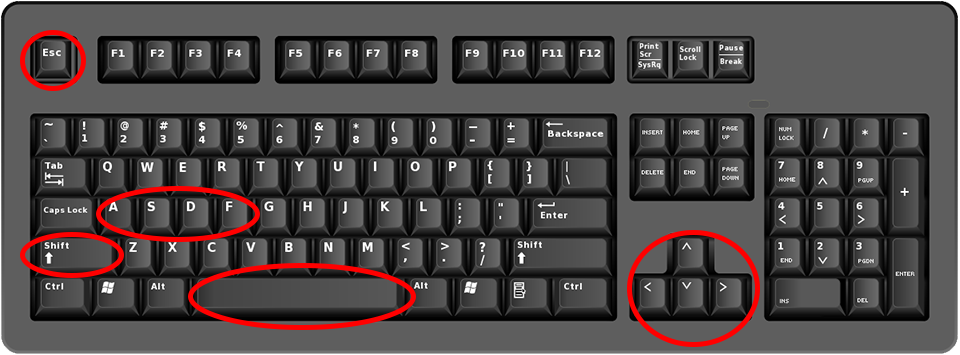
\includegraphics[keepaspectratio=true,scale=0.4]{controles.png}
\end{figure}

\begin{figure}[ht]
    \centering
    \caption{Controle via joystick}
    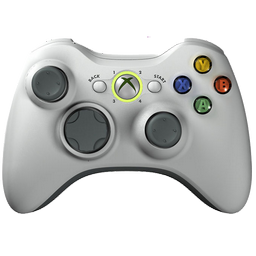
\includegraphics[keepaspectratio=true,scale=0.7]{joy360.png}
\end{figure}

\section{Contato da Equipe}
Para entrar em contato com a equipe Mana Team, por favor, envie um e-mail para: manateam.entertainment@gmail.com e responderemos tão logo pudermos.
\end{document}